\documentclass{article}
\usepackage[utf8]{inputenc}
\usepackage{amsmath}
\usepackage{graphicx}
\usepackage{pifont}
\usepackage{hyperref}
\hypersetup{
    colorlinks=true,
    linkcolor=blue,
    filecolor=magenta,      
    urlcolor=cyan,
}


\title{Raport tehnic}


\begin{document}

\maketitle

\section{Coperta}
\large{
Titlul temei: Planificarea sarcinilor \\
\\
Numele: Bucă-Ghebaură Elizabetha Alexandrina \\
\\
Grupa: CR 1.1 A \\
\\
Anul de studiu: Anul I \\
\\
Specializarea: Calculatoare și Tehnologia Informației în Limba Română 
}



\newpage
\section{Enunțul problemei}
\vspace{1cm}
Se considera p $\geq$ 1 procesoare identice și 1 $\leq$ n $\leq$ k $\times$ p sarcini de lucru, unde k este un parametru fixat, număr natural. Se cere determinarea planificării optimale a celor n sarcini pe cele p procesoare disponibile, astfel încât pe fiecare procesor să fie executate cel mult k sarcini. Se cunoaște durata de execuție $d_{i}$ a fiecărei sarcini. Se notează cu $d_{M}$=$($$\sum_{i=1}^{n}d_{i}$$)/p$ media timpului de execuție al tuturor sarcinilor pe cele p procesoare. Daca se notează cu $x_{j}$ durata cumulată de execuție a sarcinilor planificate pe procesorul 1 $\leq$ j $\leq$ p atunci planificarea optimă a sarcinilor trebuie să minimizeze dezechilibrul total față de timpul mediu, calculat prin $\sum_{j=1}^{p}|x_{j}-d_{M}|$. Se vor implementa doi algoritmi, primul pentru k=2 și al doilea pentru k=3.

\newpage 
\section{Algoritmii propuși}
\vspace{1cm}
Pentru prima metodă avem datele pe care le-am generat random, și anume numărul procesoarelor și cel al sarcinilor de lucru. Am implementat metoda MERGE SORT pentru a sorta în ordine crescătoare timpii de execuție ai fiecărei sarcini. În acest fel, pentru a doua parte a problemei unde trebuie să se  calculeze media timpului de executie,  am însumat fiecare timp de execuție al fiecarei sarcini, în final împărtind la numărul de procesoare. Mai departe, am calculat folosind o buclă durata cumulată de execuție astfel încat pe fiecare procesor să fie cel mult două sarcini de lucru. \\
\\
\hspace{1cm} \textbf{Mergesort} \\
\\
a) if (p $<$ r) \hspace{1.7cm} // avem cel puțin doua elemente \\
1. q = (p+r)/2 \\
2. mergesort(x, p, q)\hspace{1cm} // sortează x[p:q] \\ 
3. mergesort(x, q+1, r)\hspace{1cm} // sortează x[q+1:r] \\
4. mergesort(x[p:q], x[q+1:r])\hspace{1cm} // combină subșirurile \\

\begin{figure}[htp]
\centering
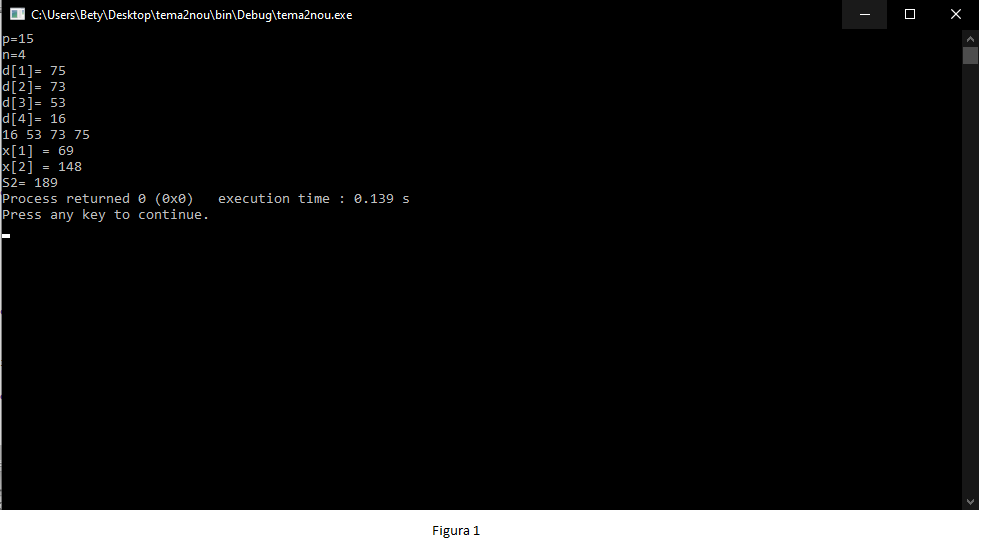
\includegraphics[width=15cm,height=8cm]{figura1}
\end{figure}
  
  Pentru a doua metodă, ca și pentru prima metodă, am folosit funcția de generare aleatorie a procesoarelor și sarcinilor de lucru. Quicksort efectuează sortarea bazându-se pe o strategie divide et impera. Astfel, el împarte lista de sortat în două subliste mai ușor de sortat. Am încercat să modific prima metodă, astfel incât pe fiecare procesor să fie executate cel mult k=3 sarcini de lucru. \\
  
 \hspace{1cm} \textbf{QuickSort} \\ 
  \\
  1. quickSort(arr[], low, high) \\
  2. if (low \textless high) \\ 
  3. pi = partition(arr, low, high) \\
  4. quickSort(arr, low, pi - 1) \\
  5. quickSort(arr, pi + 1, high) \\
    \\
 \begin{figure}[htp]
\centering
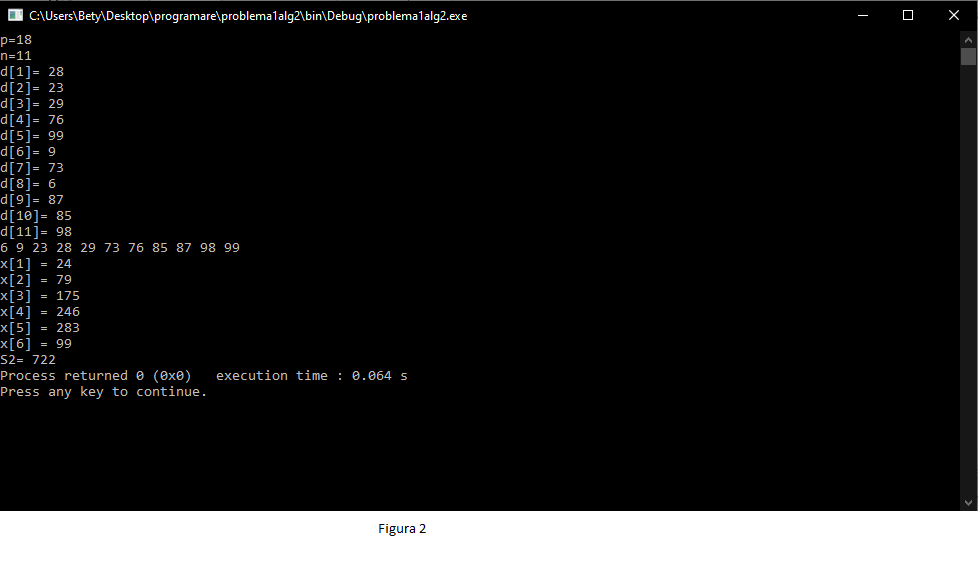
\includegraphics[width=15cm,height=8cm]{figura2}
\end{figure}
  


\newpage
\section{Date experimentale}
 Am folosit această funcție pentru a genera aleatoriu numărul de procesoare și numărul sarcinilor de lucru.  \\
 
\hspace{2cm} \textbf{Random number generator}\\

int main() \\
\big\{ \\
srand(time(NULL)); \\
int i; \\
for(i=0; i$<$7; i++) \\
printf("\%d \t", rand()); \\
return 0; \\
\big\}
\\  
\\
Funcția rand returnează un număr natural pseudo-random. Pentru a limita intervalul său de valori, putem folosi operația modulo ($\%$), așa cum am folosit-o și in algoritmul propus de mine in proiectul C.  Pentru a evita generarea acelorasi numere random la rularea programului, se folosește \emph{time(NULL)}. \\
Astfel că, în programul meu, am setat ca numărul procesoarelor și numărul sarcinilor de lucru să nu depășească 2 cifre, pentru fi mai ușor de calculat ceea ce este cerut in problemă. \\

\newpage
\section{Proiectarea aplicației experimentale}
 \textbf{ Algoritmul MergeSort}  \\
  \\
\hspace{1cm} Consideram șirul: x[1], x[2], . . . , x[n].\\
\ding{106} Se descompune șirul inițial nesortat în subșiruri de lungime 1. \\
\ding{106} Se interclasează subșirurile obținute la pasul precedent până rezultă un singur șir. \\
\\
 \textbf{Algoritmul QuickSort} \\
 \\
 \ding{106} se alege un element al listei, denumit pivot \\
\ding{106}se reordonează lista astfel încât toate elementele mai mici decât pivotul să fie plasate înaintea pivotului și toate elementele mai mari să fie după pivot; după această partiționare, pivotul se află în poziția sa finală \\
\ding{106} se sortează recursiv sublista de elemente mai mici decât pivotul și sublista de elemente mai mari decât pivotul \\

\newpage

\subsection{Structura de nivel înalt a aplicației}
\vspace{1cm}
Această figură reprezintă programul meu, prima metoda de rezolvare a problemei, cu toate sursele create; similar această schiță arată și pentru cea de-a doua metodă. \\
\begin{figure}[htp]
\centering
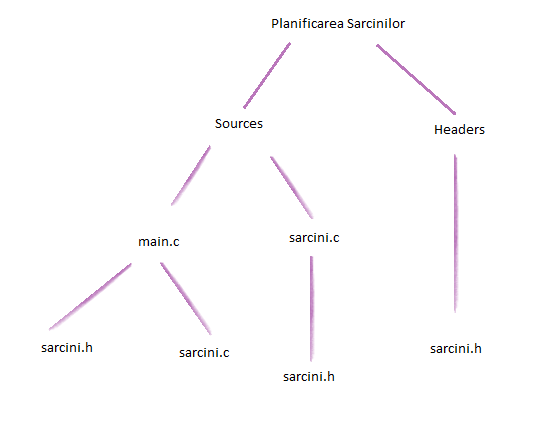
\includegraphics[width=13cm,height=10cm]{sarcini}
\end{figure}

\textbf{Apelul funcției principale}\\
Pentru metoda 1, similar și pentru metoda 2.
$\#$include $<$stdio.h$>$ \\
$\#$include $<$stdlib.h$>$\\
$\#$include $<$time.h$>$ \\
$\#$include $<$sarcini.c$>$ \\
$\#$include $<$sarcini.h$>$ \\

\newpage





\subsection{Specificarea datelor de intrare}

Am implementat prima metoda pentru a sorta crescator durata de execuție a fiecărei sarcini. \\
Datele de intrare sunt reprezentate de numărul procesoarelor și numărul sarcinilor de lucru. \\
Pentru prima metoda, din prima figura, \textbf{INPUT}-urile vor fi urmatoarele: \\
- \hspace{0.4cm}p=15 \\
- \hspace{0.4cm}n=4 \\
- \hspace{0.4cm}d[1]= 75 \\
- \hspace{0.4cm}d[2]= 73 \\
- \hspace{0.4cm}d[3]= 53 \\
- \hspace{0.4cm}d[4]= 16 \\



\subsection{Specificarea ieșirilor/rezultatelor}

Datele de ieșire sunt reprezentate de media timpului de execuție a tuturor sarcinilor, precum și dezechilibrul total din ultima parte a enunțului. \\ 
\\
 Pentru prima metoda, cea din prima figura, acesta va fi \textbf{OUTPUT}-ul: \\
 - \hspace{0.4cm}S2=189 \\


\subsection{Lista tuturor modulelor aplicației și descrierea lor}

void merge()  \hspace{1cm}// combină două subșiruri\\
void mergeSort() \hspace{1cm} // procedură recursivă care ordonează un subşir precizând limitele acestuia \\
void printArray()  \hspace{1cm}// afișează vectorul sortat \\
srand(time(NULL)) \hspace{1cm}// generează numere random
\\
void swap() \hspace{1cm} // interschimbă două elemente     \\
int partition ()   \hspace{1cm} // reordonează lista in funcție de fiecare element             \\ 
void quickSort()  \hspace{0.5cm} //  procedură recursivă care ordonează un subşir     \\



\subsection{Lista tuturor funcțiilor aplicației, grupate pe module}

\subsubsection{Descrierea scopului funcției}

Ambele metode conțin funcții care prin divizarea acestora în subprograme ajută la rezolvarea mai rapida a problemei.\\ 
\\
void merge()  \hspace{1cm}// combină două subșiruri arr[]. primul este arr[1...n]. al doilea este arr[m+1...r]\\
void mergeSort() \hspace{1cm} // procedură recursivă care ordonează subșirul arr[] \\
void printArray()  \hspace{1cm}// afișează vectorul sortat (timpul de execuție al fiecărei sarcini)\\
srand(time(NULL)) \hspace{1cm}// generează numărul procesoarelor, cel al sarcinilor de lucru și timpul de execuție pentru fiecare sarcină de lucru, random \\

\subsubsection{Descrierea fiecărui parametru}

 int p  \hspace{1cm} //  numărul procesoarelor \\
 int n \hspace{1cm} //  numărul sarcinilor de lucru \\
 int d[i] \hspace{1cm} // timpul de execuție al fiecărei sarcini de pe cele p procesoare \\
 int x[j] \hspace{1cm}// durata cumulata de execuție a sarcinilor planificate pe procesorul j \\
 
 
\subsubsection{Semnificația valorii de return}

return S2 \hspace{1cm} // returnează valoarea dezechilibrului total 
 \newpage 
\section{Concluzii}
\ding{105} Am incercat să fac ambele implementări ale algoritmilor, atât in C, cât și în Python. \\
\ding{105} În Python am întâmpinat câteva probleme, și anume niște erori pe care nu le pot desluși, din păcate nu am reușit să termin algoritmul în acest limbaj. \\
\ding{105} Am folosit algoritmul de sortare Merge Sort pentru a sorta crescător timpul de execuție al fiecărei sarcini. \\
\ding{105} Prima metoda pe care am folosit-o pentru a rezolva problema o consider optimă si mai ușoară decât a doua metodă. \\
\ding{105} Am folosit și un algoritm de generare aleatorie a numerelor, ceea ce mi-a dat puține bătăi de cap la început, însă mi-am dat seama mai târziu cum se folosește. \\
\ding{105} Pentru metoda a doua am încercat să folosesc un alt algoritm de sortare decât Merge Sort, anume Quick Sort. \\
\ding{105} Din nefericire, nu am reușit să rezolv până la capăt a doua metoda încercată, dar consider că este un început. \\
 \ding{105} De asemenea, am încercat să fac și un fișier de tip OUT, astfel încât atunci când am rulat programul, în consolă să nu apară nimic, dar să fie mutate datele de acolo în fișierul creat de mine. \\
 \newpage 
 
\section{Referințe bibliografice}

 \ding{106} \hspace{0.4cm} Chapter 6/ Capitolul 6 \\
 \ding{106} \hspace{0.4cm} \url{https://www.overleaf.com/learn} \\
 \ding{106} \hspace{0.4cm} \url{https://infogenius.ro/biblioteca-standard-c/} \\
 \ding{106} \hspace{0.4cm} Thomas H. Cormen, Charles E. Leiserson, Ronald L. Rivest, and Cliff Stein, Introduction to Algorithms (3rd edition), MIT Press and McGraw-Hill, 2009 \\
 \ding{106} \hspace{0.4cm} \url{https://www.geeksforgeeks.org/}
 







\end{document}
